\begin{equation}
u_{n\mathbf{k}}(\mathbf{r}) = \frac{1}{\Omega^{0.5}} \sum_{\boldsymbol{G}} C_{\boldsymbol{G}n\mathbf{k}}e^{i\boldsymbol{G}\mathbf{r}}
\end{equation}

\begin{equation}
\rho(\mathbf{r}) = \sum_{\boldsymbol{G}} \rho_{\boldsymbol{G}} e^{i\boldsymbol{G}\mathbf{r}}
\end{equation}

\begin{equation}
V(\mathbf{r}) = \sum_{\boldsymbol{G}} V_{\boldsymbol{G}} e^{i\boldsymbol{G}\mathbf{r}}
\end{equation} 

One method of sampling the waveform is to move the stage in a series of small steps over the time window and perform the measurement between each movement. However, this method is time-consuming as the stage needs to accelerate and decelerate and is not used in this work. To improve the speed of data acquisition, the delay stage is moved at a constant velocity and the measurement taken at regular time intervals. The lock-in uses a moving average filter to prevent data collection between these intervals, for which the length is determined by the selected time constant. This means that the sampling time interval must be longer than the filter time interval for the filter to have no effect. For an example measurement with a time constant of \SI{1}{ms}, an electrical chopping frequency of \SI{7}{kHz} and a laser repetition rate of \SI{80}{MHz}, each datapoint is constructed from approximately 1.12 million laser pulses.

\begin{figure}
    \centering
    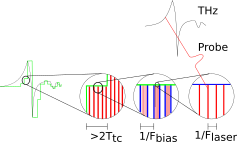
\includegraphics{Figures/Misc/Theory/THzConstituentPulses.png}
    \captionsetup{font = footnotesize, justification = centering}
    \caption{A schematic of the constituent pulses of a \acrshort{thz} waveform. It can be seen that each sampled data point is the average result of many laser pulses. \(T_{tc}\) is the lock-in time constant, \(F_{bias}\) is the electrical chopping frequency and \(F_{laser}\) is the laser repetition rate. Typical values would be \SI{1}{ms}, \SI{7}{kHz} and \SI{80}{MHz}\}.}
    \label{fig:THzPulses}
\end{figure}

\begin{figure}
    \centering
    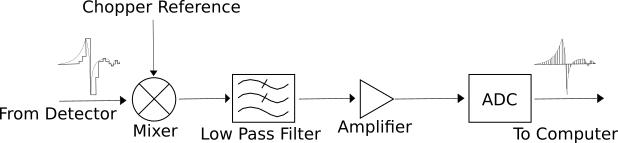
\includegraphics[scale=0.9]{Figures/Misc/Theory/LockInProcess.png}
    \captionsetup{font = footnotesize, justification = centering}
    \caption{A schematic of lock-in detection.}
    \label{fig:lockinDetection}
\end{figure}

However, the sampling period also has a maximum as without a high enough sampling frequency, aliasing can occur which distorts the signal. As the system is considered bandwidth limited, the Fourier transform of this signal is equal to zero above a selected cut-off frequency, \(F_C\). According to the Nyquist Theorem, this means that sampling at a rate of at-least twice the cut-off frequency is enough to prevent aliasing. For data processing and analysis, the data in the frequency domain must also be discrete. This is done using a discrete Fourier Transform where the bandwidth is limited by the sampling frequency. The frequency resolution is related to the length of the time window used in the measurement, however this is often fixed owing to reflections in the spectroscopic sample. This will be discussed further below. These limits place restrictions on the possible velocity of the stage and increase the measurement time.


\begin{figure}
    \centering
    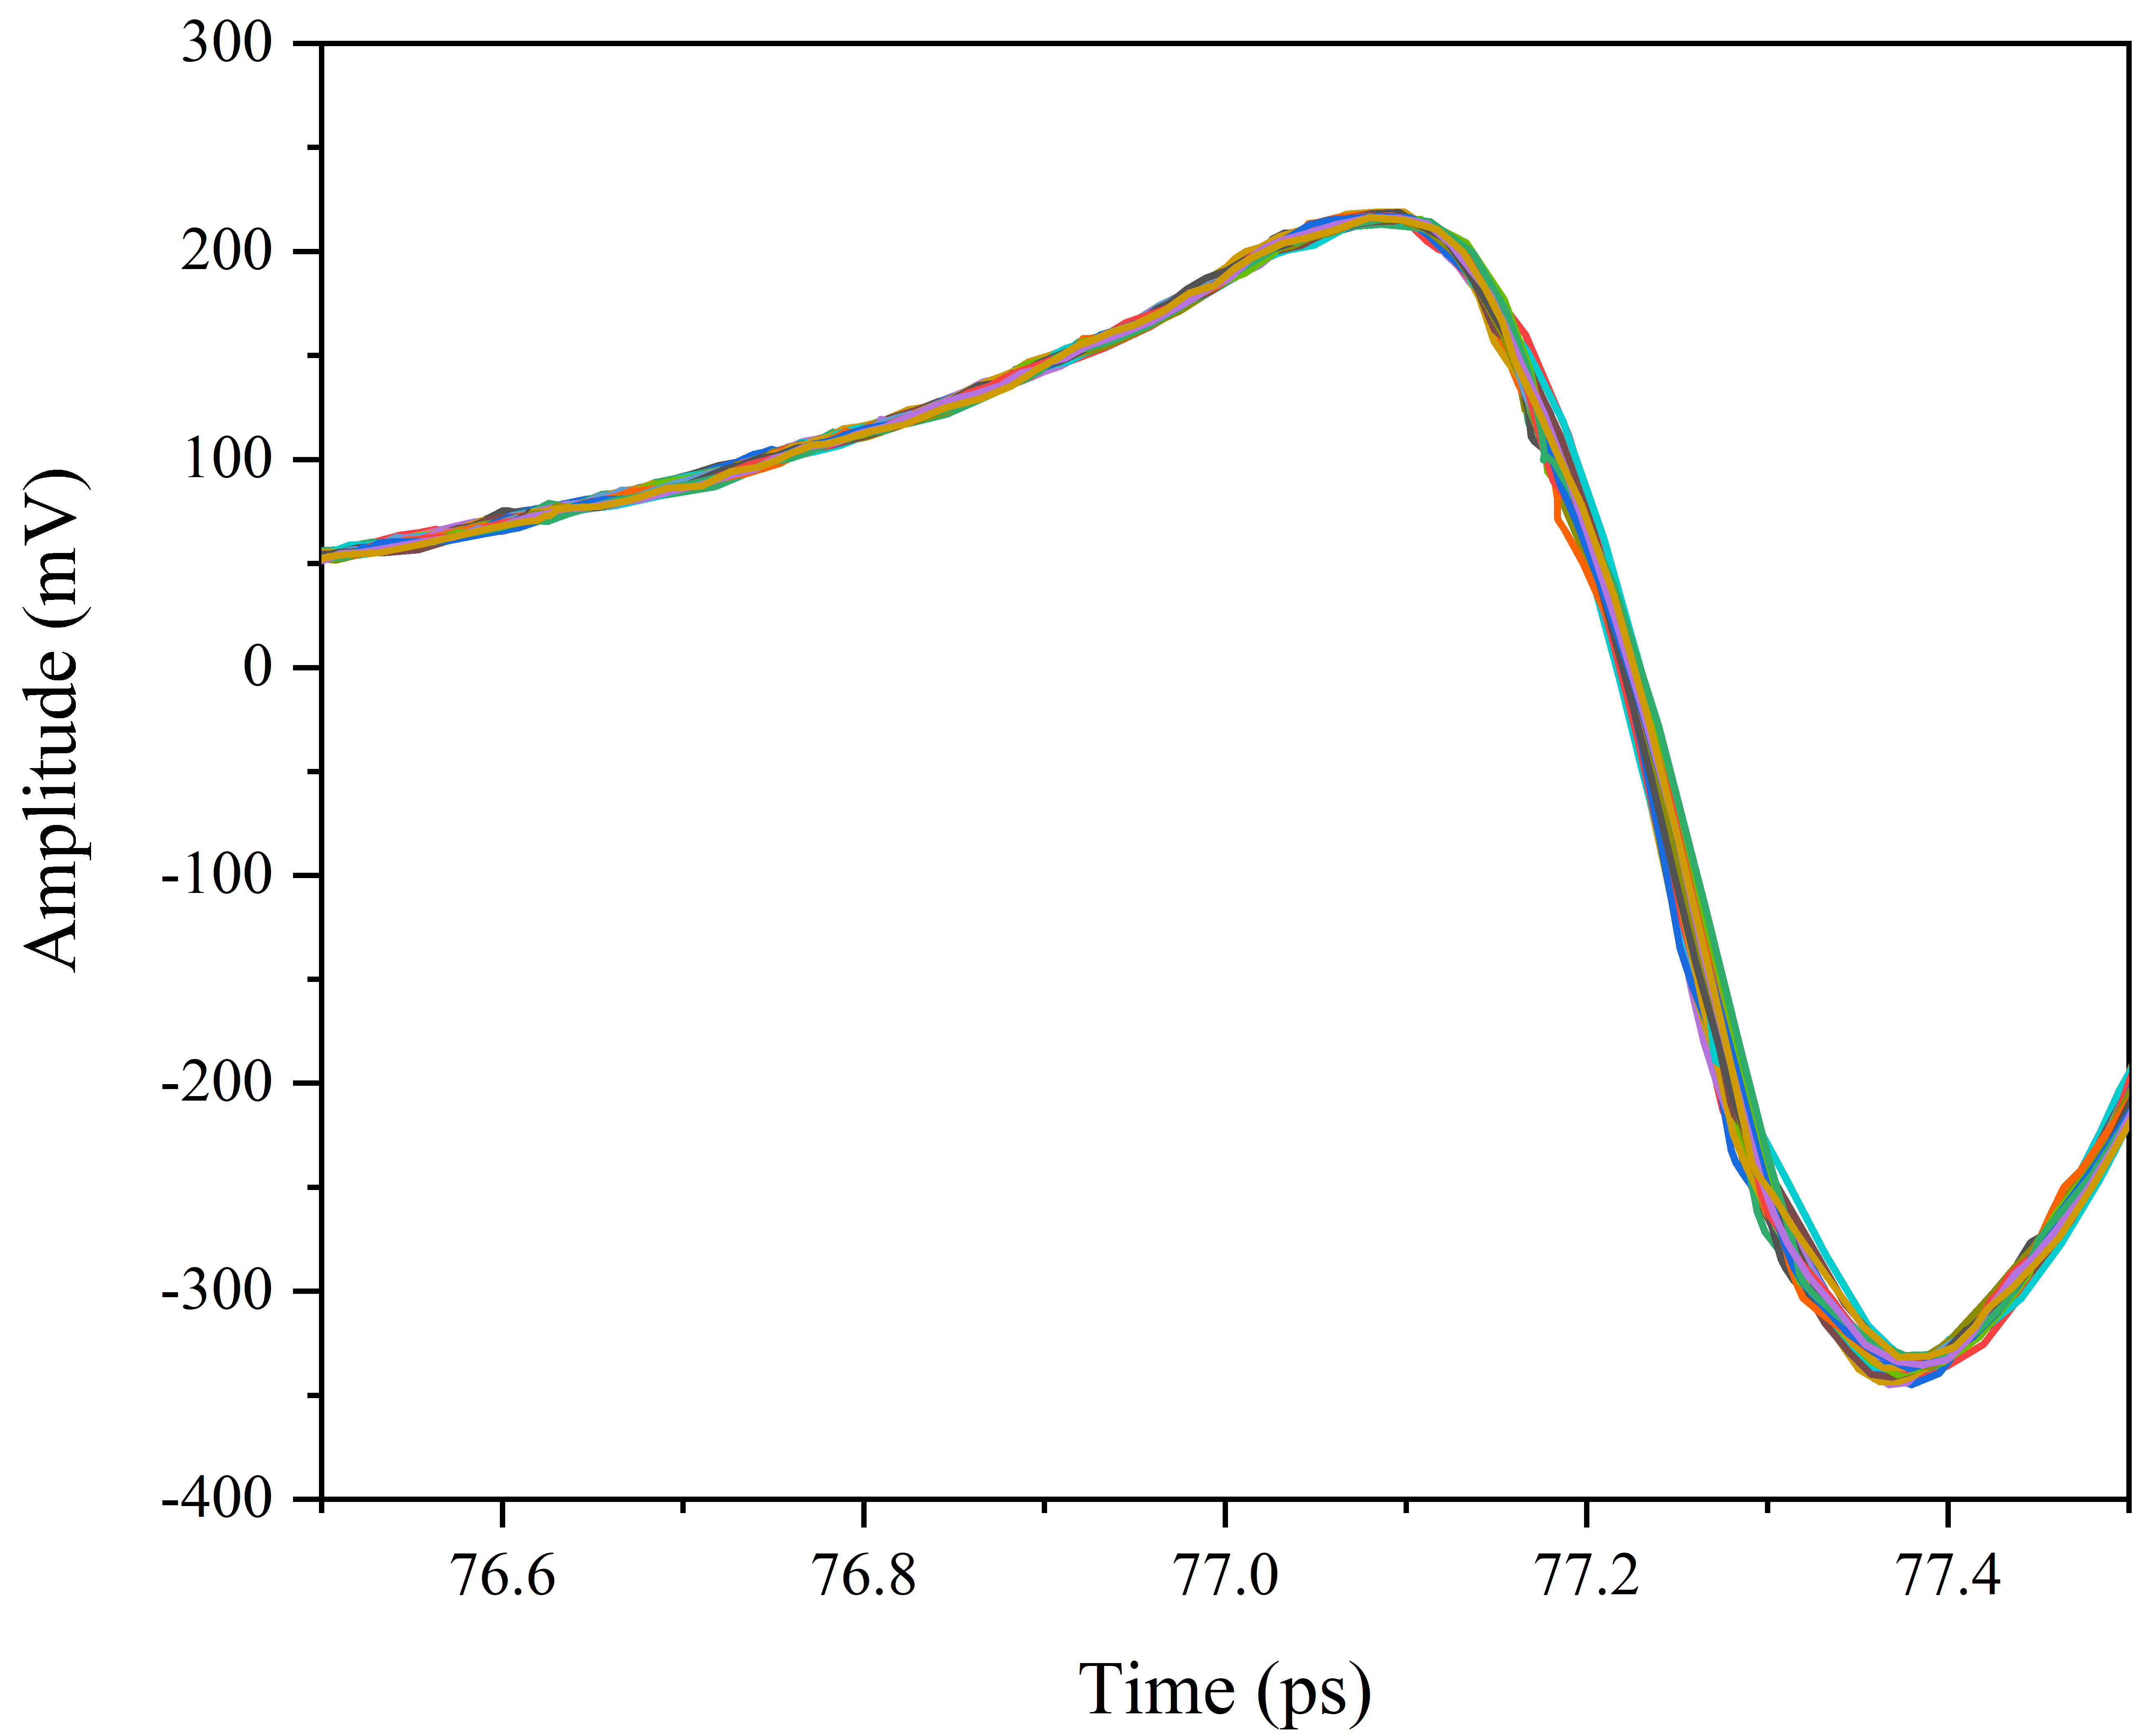
\includegraphics[scale=0.6]{Figures/Misc/Theory/AveragesG.png}
    \captionsetup{font = footnotesize, justification = centering}
    \caption{A portion of 30 individual TD traces which demonstrate the variability between each scan. 60 scans are used but 30 have been shown for clarity.}
    \label{fig:whitenoise}
\end{figure}

The detector is connected to the lock-in, which takes the chopping frequency as a reference and the detector output and demodulates the signal, where it is passed through a low-pass filter and finally sampled using an analogue-to-digital converter (ADC). This converts the signal from continuous to discrete data and this can be stored by a computer as shown in \Cref{fig:lockinDetection}.

\subsection{Transfer Functions for THz-TDS}
A Linear Time-Invariant (LTI) system has a linear relationship between its input and output which is not dependent on time. The input can be a reference \acrshort{thz} measurement, which will be dry air that the sample will displace, and the output can be a sample \acrshort{thz} measurement. Both variables are dependent on time, with their relation being some function, \(F\). In the case of an LTI system this can be written as convolution operation: 

\begin{equation}
y_t = F * x_t = (x * h)_t = \int_{-\infty}^{\infty} (x_{\tau} h_{(t-\tau)}) d\tau
\end{equation}

Where \(h\) is the impulse response of the system which is a quantitative description of the sample’s interaction with the THz radiation. Representing convolution in the TD as multiplication in the FD can be done using the Convolution theorem: 

\begin{equation}
F^{-1} (X_{\omega}Y_{\omega}) = F^{-1}(F(x_t)F(y_t)) = x_t * y_t
\end{equation}

Where \(F\) is the Fourier Transform, \(F^(-1)\) is the inverse Fourier Transform, \(X_{\omega}\) is the frequency dependent input signal and \(x_t\) is the time dependent input signal. \(Y\) represents the output signals.  This can be used with regards to an LTI by representing the output spectrum, \(Y_{\omega}\), as multiplication of the input spectrum, \(X_{\omega}\), with the transfer function \(H\): 

\begin{equation}
Y_{\omega} = X_{\omega} H_{\omega}
\end{equation}

The transfer function is the Fourier transform of the impulse response. This can be used to deconvolve an impulse response of a system with known input and output:

\begin{equation}
h_t = F^{-1}(H_{\omega}) = F^{-1}\left(\frac{Y_{\omega}}{X_{\omega}}\right)
\end{equation}

The simplest form of electromagnetic (EM) wave is a sinusoidal electric wave with a sinusoidal magnetic wave oscillating in the perpendicular plane. The magnetic component is assumed to have effectively zero interaction with a dielectric, and thus can be ignored. These waves can be modelled as plane waves, where the phase of the wave is constant over the plane perpendicular to the direction of travel and this definition is primarily used. However, it is more accurate to model the wave as having a Gaussian intensity distribution in this plane but this too can be modelled as a plane wave in the region of focus.

These can be thought of as a multitude of simple harmonic oscillators representing the chemical bonds where the relative displacement of the charges creates the dipole that interacts with the incident radiation. At \acrshort{thz} frequencies, these are largely intra-molecular interactions which can be challenging to identify without supplementary theoretical simulation. This is further complicated through other effects such as thermal broadening \cite{Walther2000} and scattering \cite{Franz2008}, which can be difficult to incorporate into theoretical calculations.

This relies on several key assumptions for the sample and the \acrshort{thz} beam. The sample is assumed to be a non-conducting dielectric cuboid which has a constant refractive index and an identical magnetic permeability to dry air whilst the \acrshort{thz} beam is assumed to be collimated. In this model, the beam travels in the direction perpendicular to the sample’s surface. These assumptions are valid when the thickness of the sample is comparatively small compared to the focal length of the parabolic mirrors used to collimate the \acrshort{thz} beam. When using thicker samples, the Gaussian beam profile provides a more suitable assumption \cite{Kuzel2000}. 

As the wave enters the material it is slowed down owing to the increased relative permittivity of the material which manifests as a decrease in wavelength and attenuated through interaction with the electric field of the system.

The left and middle terms of the equation have boundaries between \(\pi\) and \(-\pi\) as they are complex exponentials, but the right term does not. This means that the phase must be ‘unwrapped’. This is the process of adding multiples of \(2\pi\) whenever the angle passes over a boundary. This is where the sampling rate of the system becomes critical, as if the sampling period is too low then the phase will be incorrectly wrapped, as shown in \Cref{fig:aliasing}. As the unwrapped phase underpins the calculation of the refractive index and permittivity, it is vital that the sampling frequency is high enough that aliasing does not occur.

\begin{figure}
    \centering
    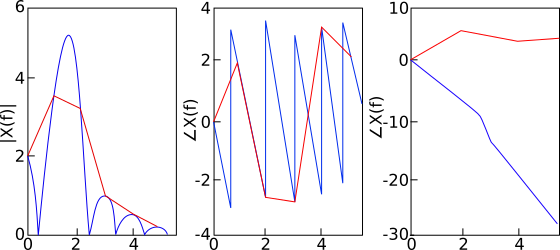
\includegraphics{Figures/Misc/Theory/AliasingMagPhase.png}
    \captionsetup{font = footnotesize, justification = centering}
    \caption{Magnitude as a function of frequency, b) wrapped phase and c) unwrapped phase. These diagrams show the effect of sampling frequency. The red line corresponds to a low sampling frequency and the blue line corresponds to a high sampling frequency. The effect on the unwrapped phase, from which the refractive index is calculated, is evident. Additionally, sharp spectral features in a magnitude spectrum can also be missed.}
    \label{fig:aliasing}
\end{figure}

From which the absorption coefficient can be calculated. This is a form of the Beer Lambert Law. The absorption spectra that are produced can be extremely difficult to interpret owing to the vast array of long-range interactions in a crystal. There is the additional issue that owing to fluctuations in humidity, temperature, sample consistency and laser power, repeat measurements can have significant variations. This increases the system noise, which lowers the SNR and this can obscure features on the spectrum. Finally, scattering is also a significant problem owing to the wavelength of \acrshort{thz} light, which further reduces the SNR, particularly at higher frequencies (>\SI{3}{THz}).

\subsubsection{Gaussian Beam Effects}
This model is suitable for relatively thin samples, but when the samples reach a significant thickness it is no longer applicable. As mentioned above, it is more accurate to model the \acrshort{thz} beam as having a Gaussian profile. This results in the sample acting as a weak lens on the \acrshort{thz} beam, adjusting its focus as shown in \Cref{fig:guoy}.
This can be problematic as the ideal reference alignment involves focusing the beam onto the detector, and when the sample measurement is taken the focus will have moved into the detector, reducing the amplitude and the SNR. In addition, the phase will now be incorrect as the \acrshort{thz} has propagated through a thicker portion of the sample than in the model. This is known as Gouy phase shift and means that a phase correction must be applied to extract accurate spectroscopic parameters. As \(\Delta\) does not vary to much extent it is often permitted to use a pre-calculated correction which was created from a calibration model. 

\begin{figure}
    \centering
    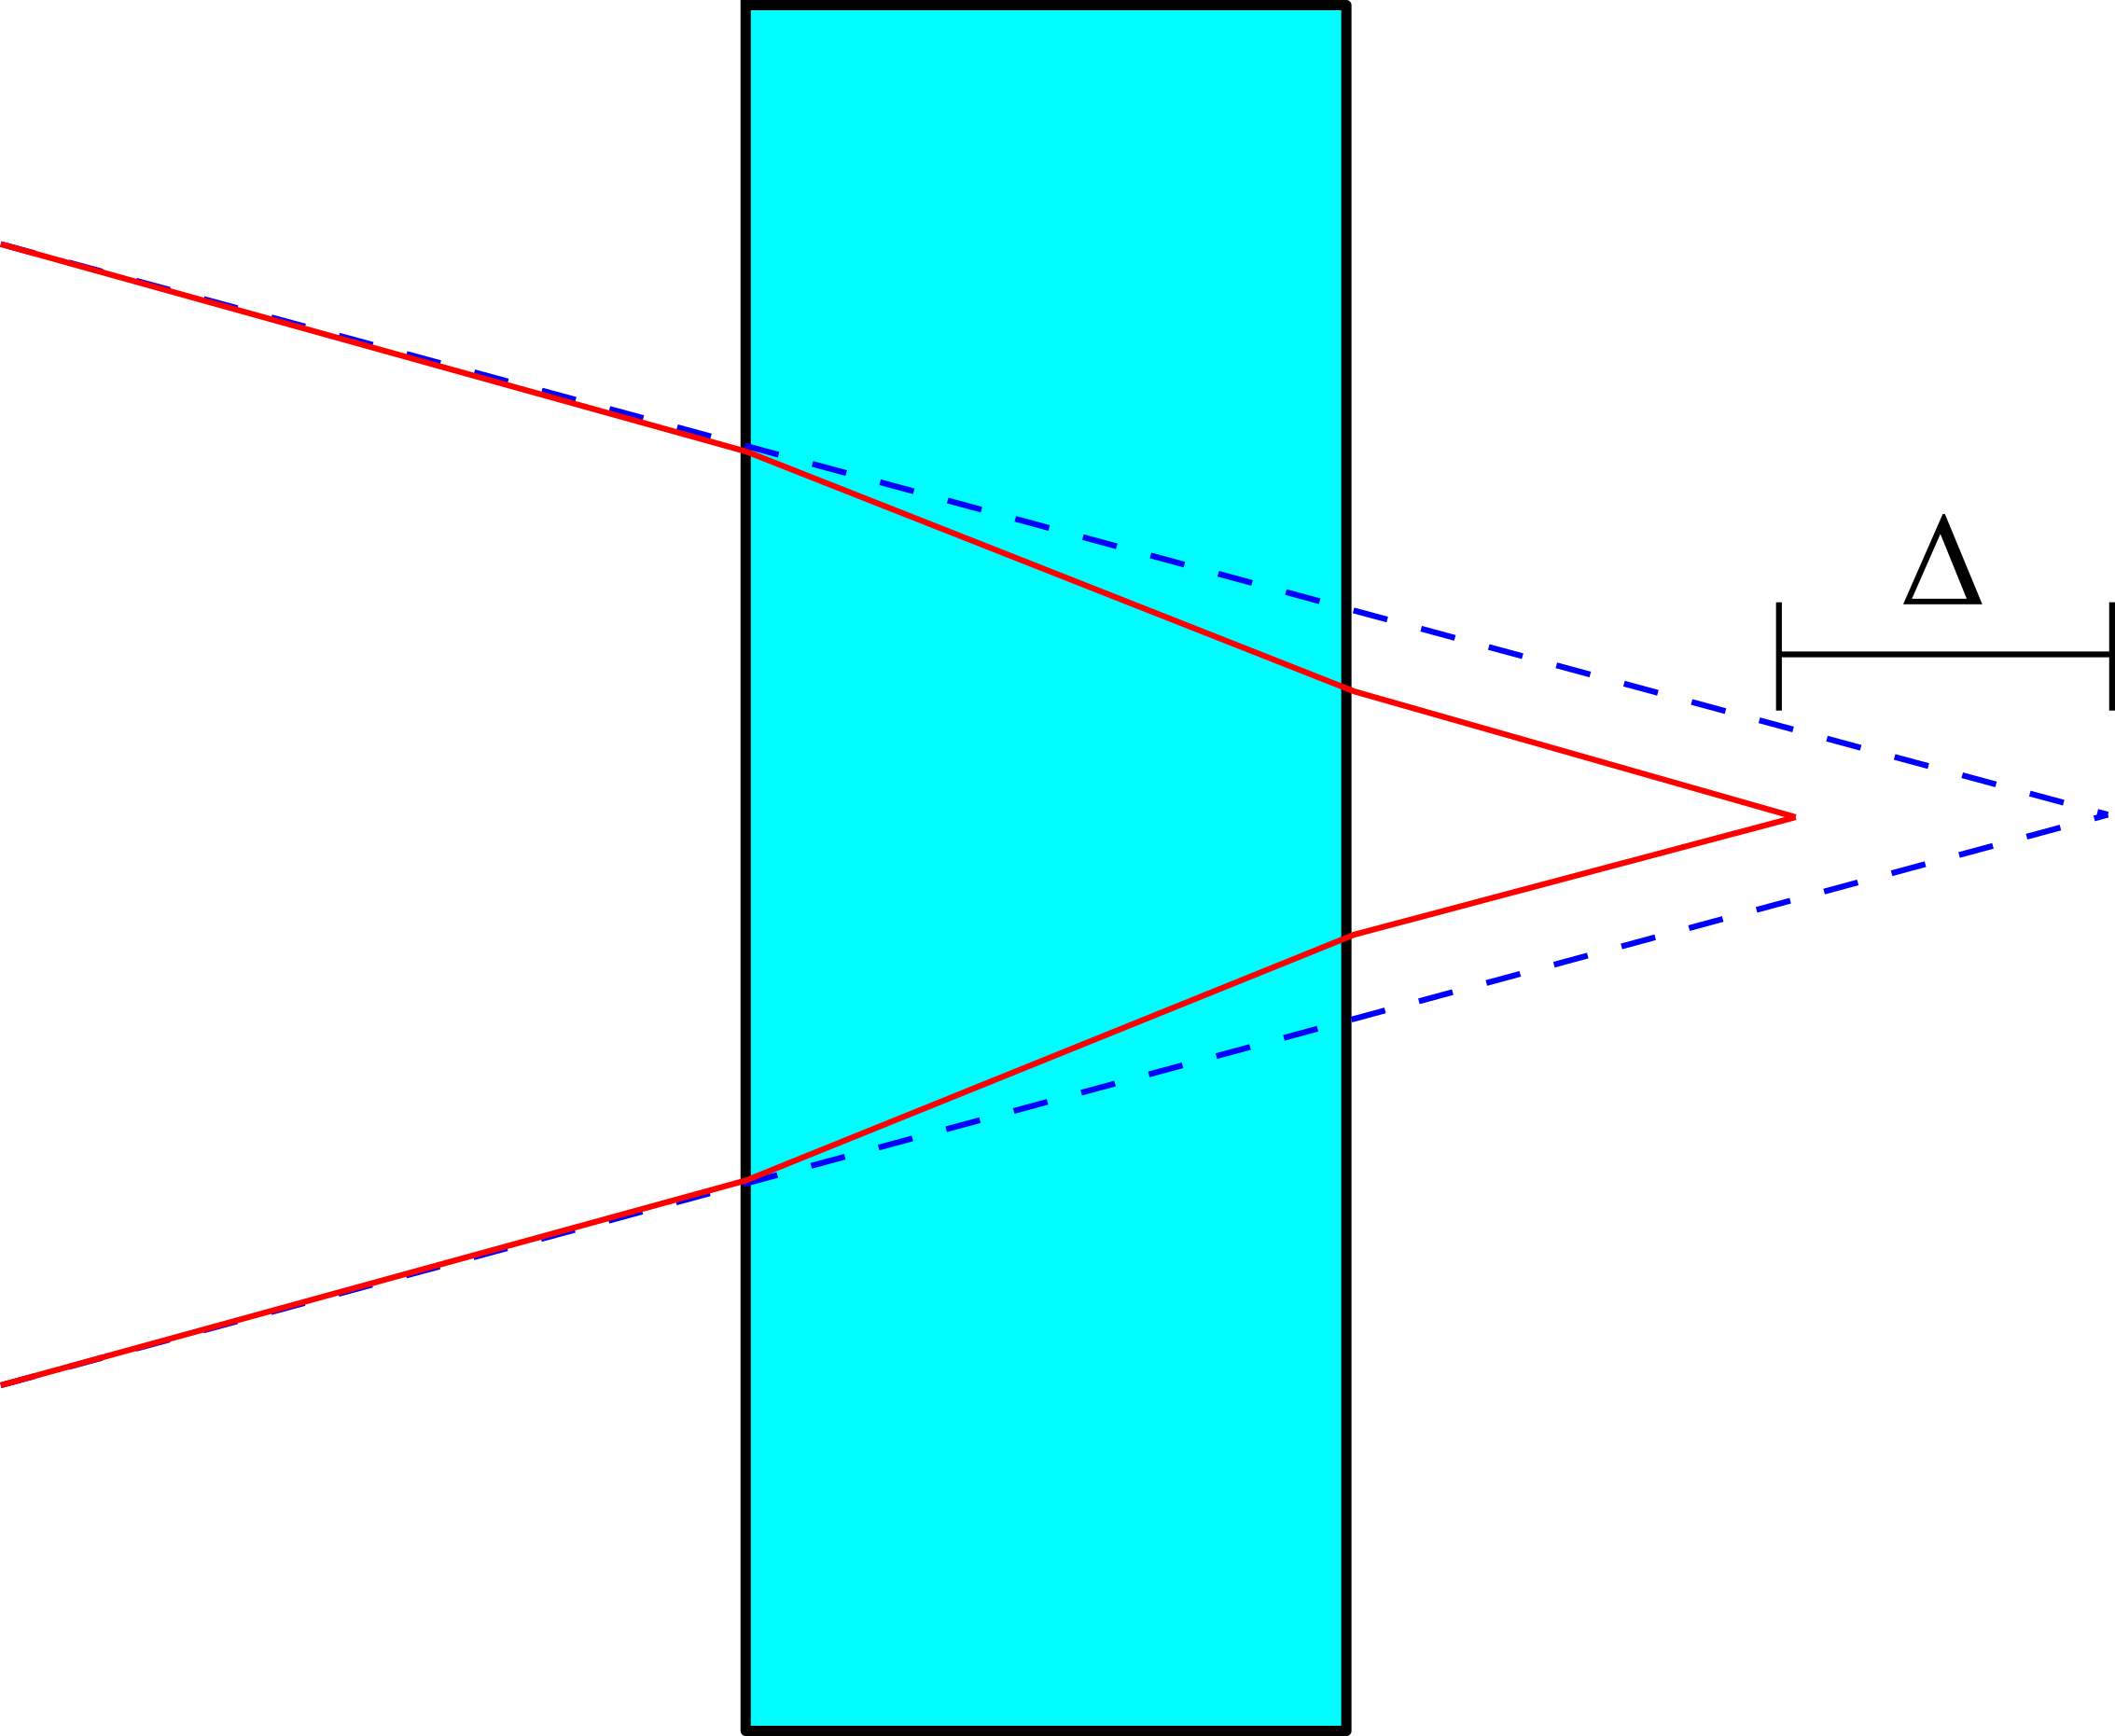
\includegraphics{Figures/Misc/Theory/GuoyPhaseShift.png}
    \captionsetup{font = footnotesize, justification = centering}
    \caption{A schematic showing how the \acrshort{thz} beam is focused by the sample, causing a shift of \(\Delta\). This results in less signal, reducing SNR, and increases the error in extracted parameters as the effective thickness has increased.}
    \label{fig:guoy}
\end{figure}

This calibration is performed using a sample with a distinct echo such as thick sapphire substrate. By using the methods described above to window the two pulses separately, the transfer function for each can be calculated and the refractive index for each pulse extracted. The parameter \(\beta\) is used in this work to describe all gaussian beam effects causing this difference, and its relationship to refractive index is described by:

\begin{equation}
\beta = \frac{3}{2}(n_0 - n_1)
\end{equation}

Where \(n_0\) and \(n_1\) are the original pulse and first reflection respectively. If this correction is not included then incorrect estimates for the thickness, and therefore refractive index, will be obtained. This is demonstrated in \Cref{fig:guoythickness}, where it can be seen that the thickness extraction process described above has different extracted thicknesses. Additionally, it can be seen that there is less total variance when the correction is included, which results in cleaner spectra for interpretation. 

\begin{figure}
    \centering
    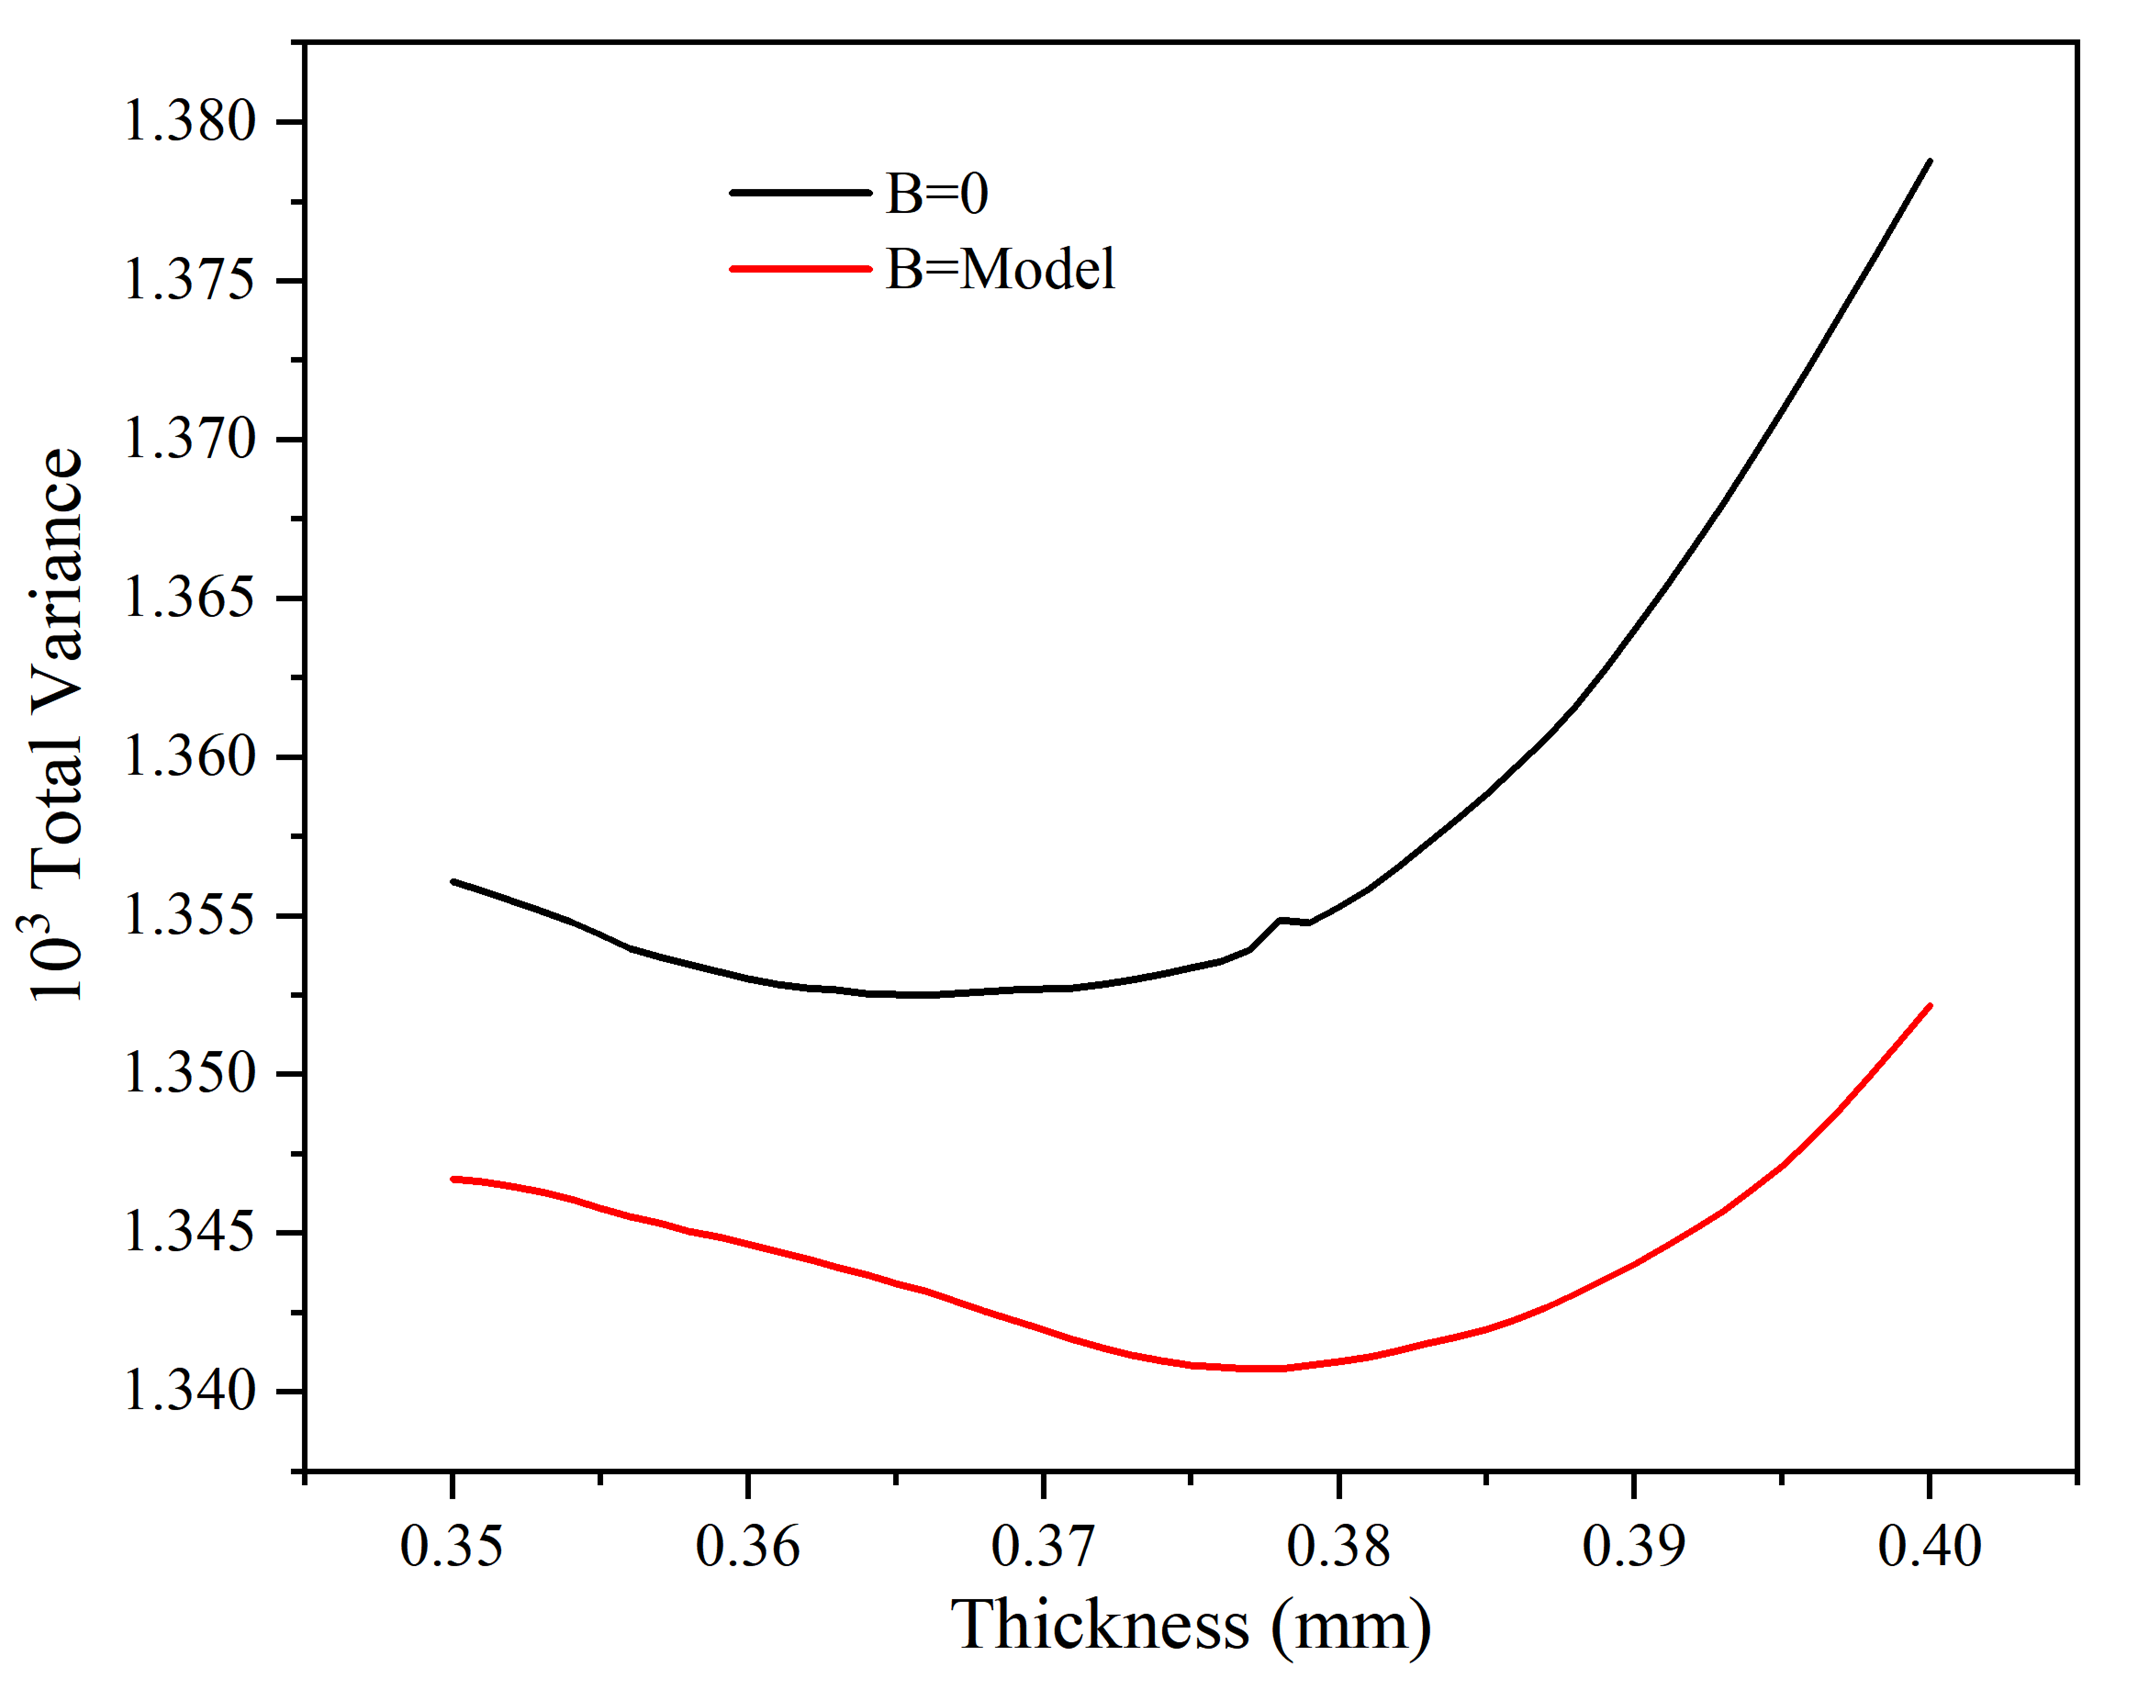
\includegraphics{Figures/Misc/Theory/guoythickness.png}
    \captionsetup{font = footnotesize, justification = centering}
    \caption{The thickness extraction curves for no correction (black) and calibration model (red). The model has improved thickness extraction accuracy and decreased total variance in the spectrum.}
    \label{fig:guoythickness}
\end{figure}

This leads to uncertainty in the frequency of a mode and can be particularly problematic when spectral features are in close proximity. The simplest window function is rectangular, but this can cause problems in the frequency domain such as frequency leakage which increases the uncertainty in the frequency component \cite{Popescu1996}.

System reflections should cancel out but they do not, owing to the difference in temporal separation between the reflection and the relative pulses and delay stage jitter and poor SNR at high frequencies.  The time window is first applied to the reference measurement. As the sample measurement can be assumed to be a delayed, attenuated approximation of the reference, they can be cross-correlated to calculate the delay between the pulses as the maximum of this function corresponds to when the measurements have the greatest degree of overlap. This can then be applied to the window for the sample measurement, as long as systematic reflections have been removed from both scans. The frequency spectrum’s resolution can be increased by artificially increasing the length of the scan. This is done through adding zero-valued datapoints to the end of the dataset. As such, it is referred to as the computational resolution or ‘zero padding’ and is mathmatically equivalent to applying a smoothing filter in the frequency domain.

The VASP DFT package was used to optimise the atomic positions and unit cell dimensions of $\alpha$LM, which was obtained from the Cambridge Crystallographic Database11. The Projector Augmented Wave12 (PAW) pseudo-potentials, distributed with VASP 5.4.4., were used to efficiently calculate the wavefunction close to the nuclei. The chosen functional was the \acrshort{pbe} functional. Each calculation used the Monkhorst-Pack14 method for the description of k-points.

\begin{table}[h]
\centering
\begin{tabular}{@{}cccccccccccc@{}}
\toprule
Peak & 1 & 2 & 3 & 4 & 5 & 6 & 7 & 8 & 9 & 10 & 11 \\ \midrule
    & 0.6 & 0.6 & 1.0 & 0.8 & 2.0 & 0.8 & 1.5 & 0.9 & 2.7 & 1.2 & 1.0 \\ \bottomrule
\end{tabular}
\caption{The FWHM experimental peak widths extracted from \Cref{fig:aLM_abs_gaussian}}
\label{tab:fwhm}
\end{table}

When exciting each device with 80 fs wide pulses at a frequency of 780 nm, they demonstrated that the SI-GaAs device outputted significantly more power than that of the LT-GaAs when biased below 30 V, attributed to the high mobility carriers in SI-GaAs. Daves Paper, may explain GaAs higher performance at these low carrier densities.

% https://refractiveindex.info/?shelf=main&book=GaAs&page=Aspnes it tells you the transmittance

1st batch was 3x100 and 3x10 sapphire - are we including the 100s?
2nd batch was 1 x 5, 10, 20, 40 sapphire 
3rd batch was 2 x 5, 10, 20, 40 gaas
4th batch was 1 x 5, 10, 20, 40 sapphire
5th batch was thick sapphire substrate 100 but josh tested those not me.
6th batch was the 3 x 20 emitters on a single substrate. These were broken when trying to remove and restick but cant remember if I got data on one before it blew up. Dont seem to have it on my computer but will go and double check on lab computer.

\begin{figure}[ht]
\centering

\begin{subfigure}{0.49\textwidth}
\centering
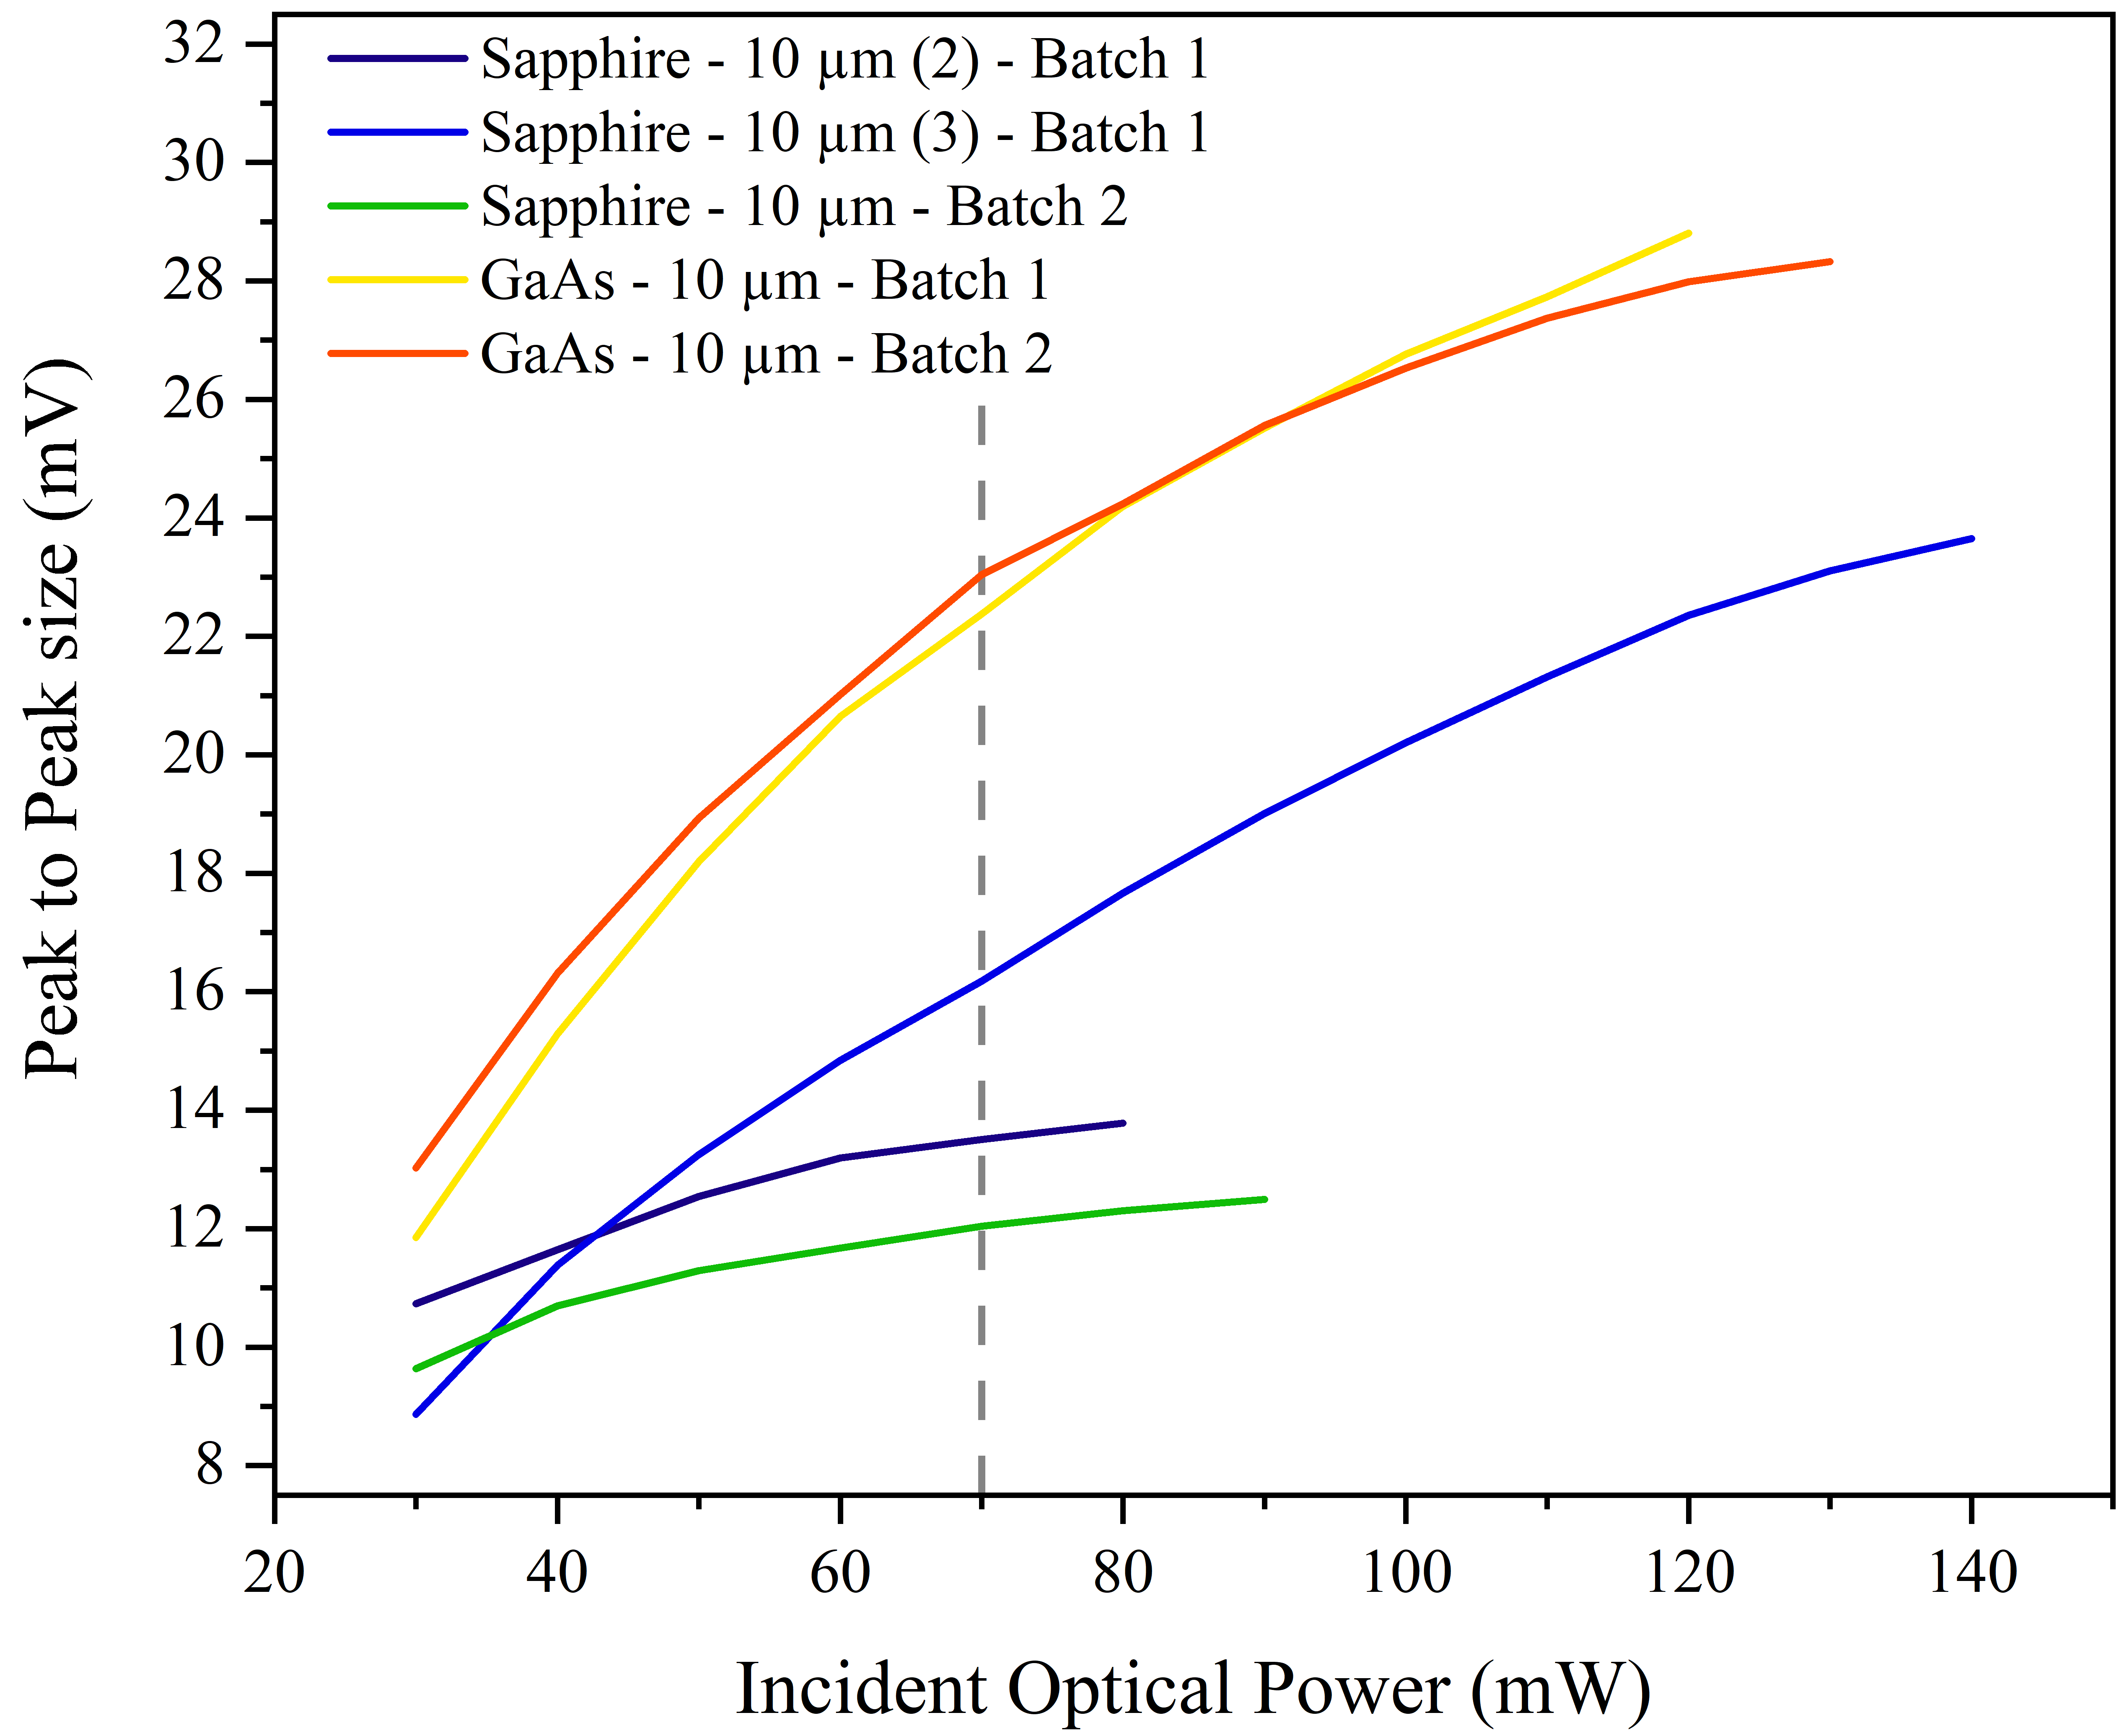
\includegraphics[width=\textwidth]{Figures/Misc/SysDev/Opt10micronG.png}
\caption{The peak to peak signal values for all devices with a gap size of \SI{10}{\micro\metre}. There is disagreement between the sapphire batches but saturation behaviour and output are consistent within batches.}
\label{fig:10micron}
\end{subfigure}
\begin{subfigure}{0.49\textwidth}
\centering
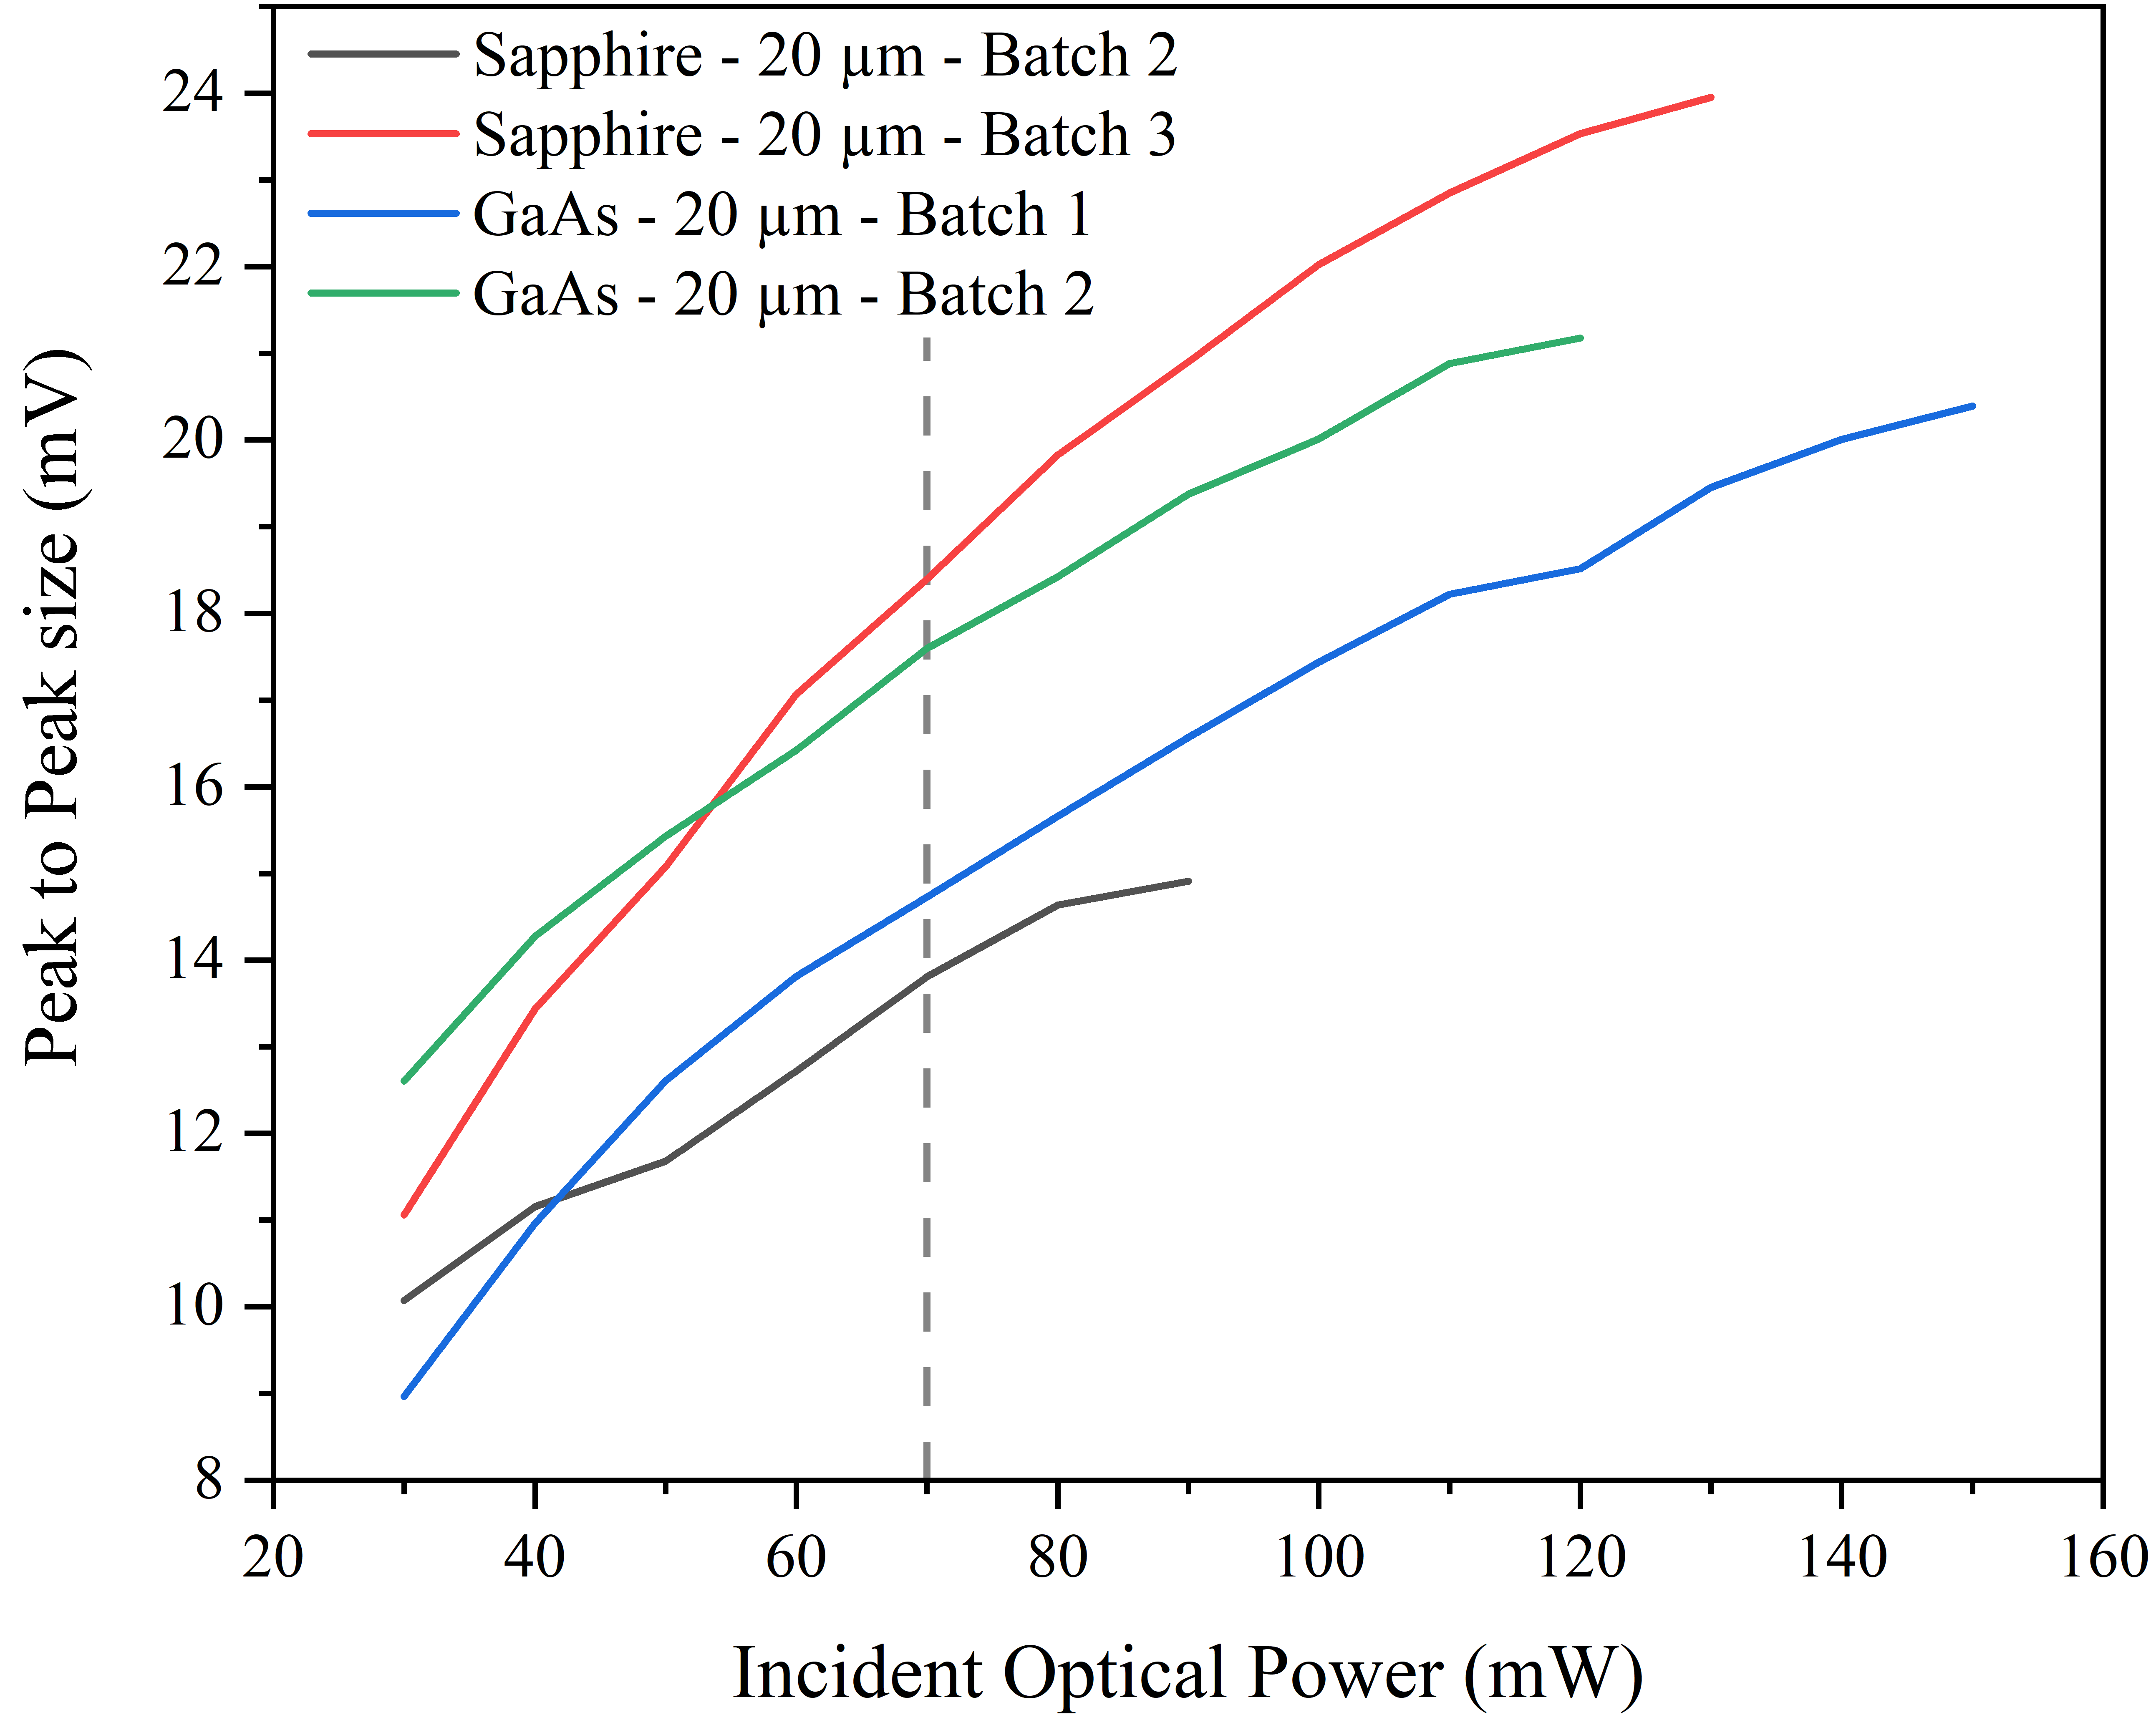
\includegraphics[width=\textwidth]{Figures/Misc/SysDev/Opt20micronG.png}
\caption{The peak to peak signal values for all devices with a gap size of \SI{20}{\micro\metre}. The sapphire devices show significant disagreement.}
\label{fig:20micron}
\end{subfigure}

\begin{subfigure}{0.49\textwidth}
\centering
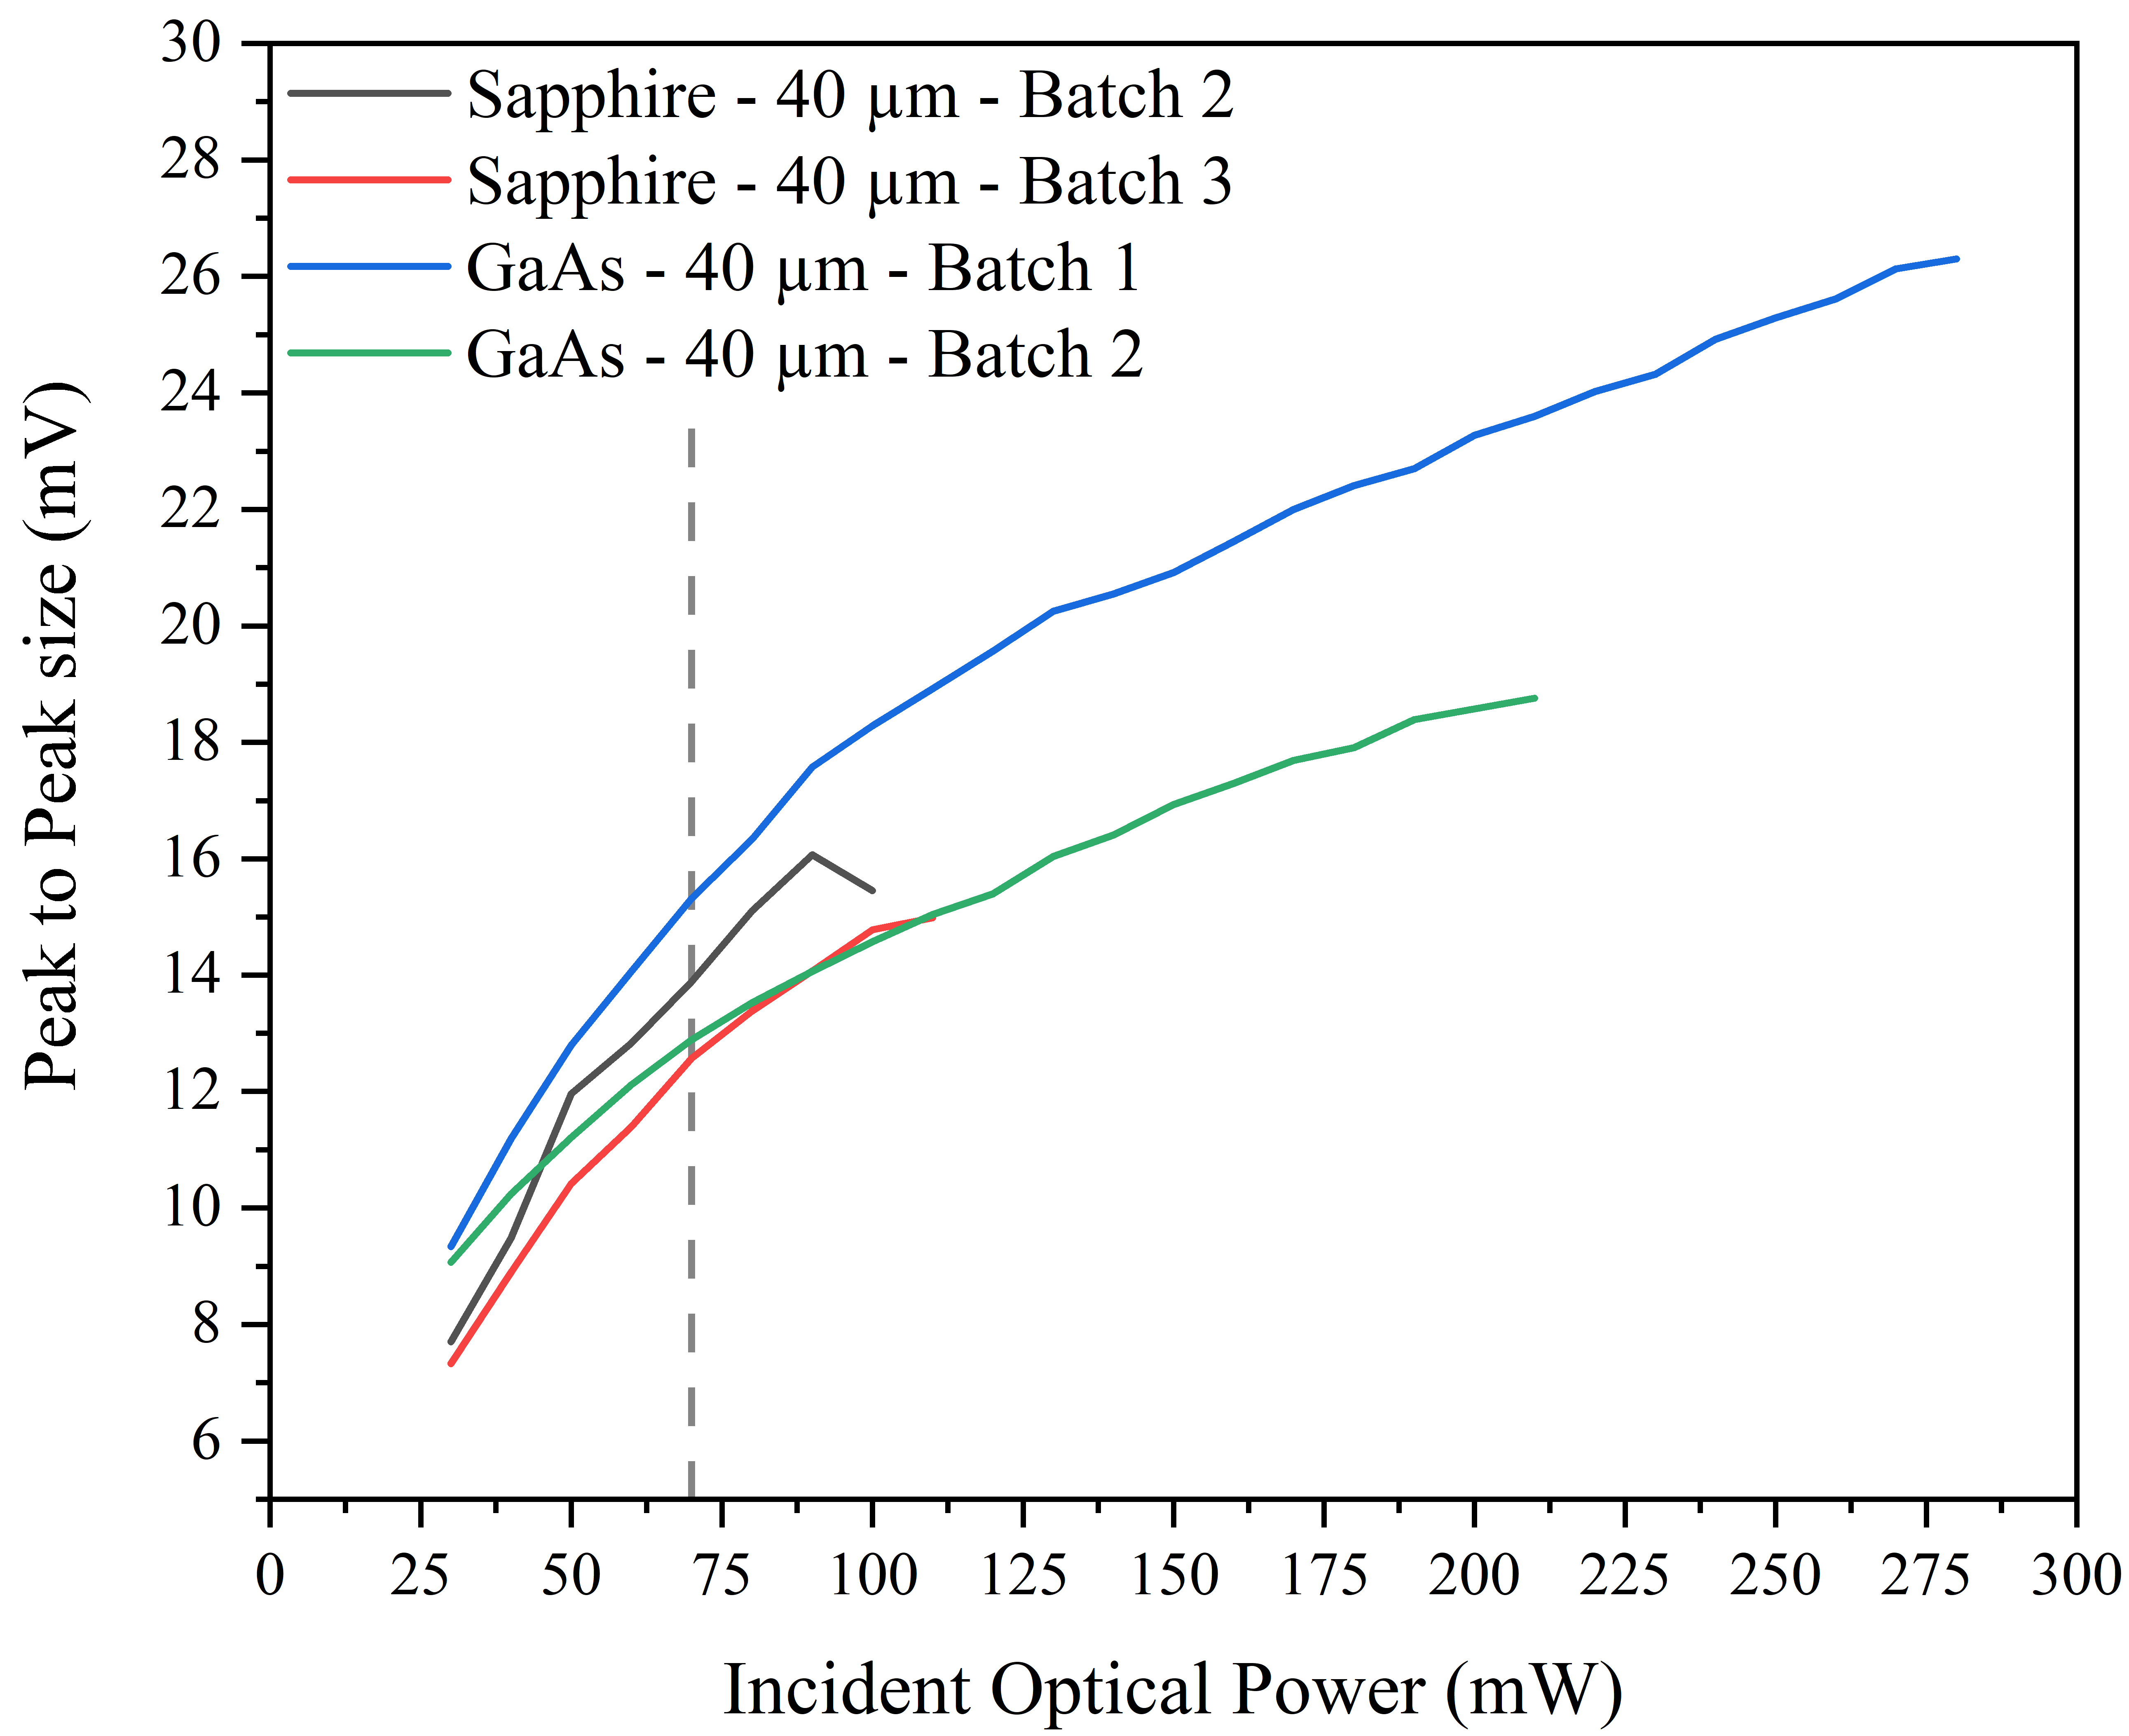
\includegraphics[width=\textwidth]{Figures/Misc/SysDev/Opt40micronG.png}
\caption{The peak to peak signal values for all devices with a gap size of \SI{40}{\micro\metre}. The sapphire devices saturate much earlier than expected when compared to their GaAs counterparts.}
\label{fig:40micron}
\end{subfigure}

\captionsetup{font = footnotesize, justification = centering}
\caption{The peak to peak signal values for all devices.}
\label{Fig:102040micron}
\end{figure}

%The application of a frequency scalar yields a comparable spectrum to experiment, but upon closer inspection it is found to move the lowest absorption feature (experimentally at 0.74 THz) well out of agreement, indicating that particular mode is well-modeled by the harmonic approximation. This helps to confirm the hypothesis that the lack of any significant shifting for that feature is a result of its harmonic nature



An examination of the step by step changed in energy and force reveal that an examination of our calculation criteria and method could result in much more consistent calculation results and a dramatic increase in speed, something that will be vital for projects such as temperature dependent spectra and electron rich molecules which typically take extensive time periods. 

%Vibrational relaxation can be incredibly complex, with motions propagating through hundreds, to even thousands, of atoms within very short time periods (<1 ps).7,8 Despite this, the fundamental origins of these relaxation pathways can be traced to the anharmonicity of individual vibrations, a property that allows for coupling between two (or more) modes.9−12 

%Anharmonic Coupling of Stretching Vibrations in Ice: A Periodic VSCF and VCI Description Ref this somewhere

